\chapter{Secure Device Identity}


A secure device identifier (DevID) is defined as an identifier that is cryptographically bound to a device \cite{DevIDSpec-IEEE}. A DevID must not be transferable from one device to another and must be stored in a way that protects it from modification. Since the TPM is a secure Root of Trust for Storage and protects keys against compromise, TPM keys are an ideal choice for DevIDs. 
The binding of a TPM key to a specific device instance is represented by a DevID certificate.
To know when and by whom DevIDs are typically created, it is useful to briefly consider a simplified version of the process for creating and distributing TPM-containing devices to end users.
\begin{enumerate}
  \item\label{ite:idTPM} TPM Manufacturers produce TPM chips according to the international standard. They provision each TPM chip with an EK certificate which binds the EK to a specific TPM. These chips are then distributed to the original equipment manufacturers (OEMs).
  \item\label{ite:idDevIni} OEMs produce devices (e.g., PCs) with these TPM chips integrated. They provision each TPM chip with one or more DevID certificates which bind a key to a specific device. These devices are then distributed to the end users (Owners).
  \item\label{ite:idDevLoc} Owners may optionally provision their TPM chip with one or more DevID certificates which bind a key to their specific device.
\end{enumerate} 

The provisioning of device identification in Steps \ref{ite:idDevIni} and \ref{ite:idDevLoc} is the primary subject of this work. It is important to note that an EK is not a DevID because its associated certificate identifies a TPM not device. 
%A device with TPM-based DevID capabilitities includes at least one Initial Device Identifier (IDevID).  An IDevID is intended to be long-lived and usable for the lifetime of the device. IDevIDs are installed by OEMs in TPM-containing devices at manufacturing time. Additionally, a device with DevID capabilitities may support the creation of Locally Significant Device Identifiers (LDevIDs) by the end user (i.e., the Owner). LDevIDs are not expected to be long-lived because an Owner may create new LDevIDs as often as they need.
%An LDevID must not be transferable to a device with a different IDevID without knowledge of the private key used to produce the cryptographic binding. 
When using a TPM key for secure device identity, there are restrictions on the attributes that it can have in order to enforce the best security practices. The \verb|Sign| attribute must be set and the \verb|Decrypt| attribute not set. This is in fact another reason that an EK cannot be a DevID --- recall from Section 2.1 that EKs are storage keys and therefore have the \verb|Decrypt| attribute set. Furthermore, a DevID must have the \verb|FixedTPM| attribute set because it is of paramount importance that it never be duplicated, transferred, or copied. On the other hand, the \verb|Restricted| attribute is optional. When the \verb|Restricted| attribute is set, such a key is called an attestation key (AK). This DevID gets its special name due to its unique ability to prove that some object or data is contained within the same TPM as itself. The acronyms DevID and AK are prefixed by the letter I or L denoting Initial or Locally Significant respectively. Initial device identifiers are installed by OEMs in TPM-containing devices at manufacturing time; IAKs and IDevIDs correspond with the keys referenced in Step \ref{ite:idDevIni}. Initial device identifiers are intended to be long-lived and usable for the lifetime of the device. Since an Owner cannot provision new Initial device identifiers, these keys should be recoverable to avoid the loss of these essential identifiers. Primary keys can be recreated during the lifetime of the TPM. Therefore IAKs and IDevIDs should be Primary keys. Locally Significant device identifiers are installed by Owners; LAKs and LDevIDs correspond with the keys referenced in Step \ref{ite:idDevLoc}. Locally Significant device identifiers are not expected to be long-lived because an Owner may install new ones at any time. 


%The acronym AK is prefixed by the letter I or L denoting Initial or Locally Significant respectively.  OEM-installed DevIDs (i.e., IAKs and IDevIDs) should be Primary keys so that they may be recoverable by the Owner. Since an Owner cannot provision new IAKs or IDevIDs on their device, these keys should be able to be recreated during the lifetime of the TPM or more precisely during the lifetime of the TPM’s Primary Seed to avoid the problematic loss of these essential identifiers. 
\begin{table}[h]
  \begin{center}
    \scriptsize 
    \sffamily
    \renewcommand{\arraystretch}{1.5}
    \begin{tabular}{ |c|c|c|c|c|c|c| }
      \hline
      Key & Type & \verb|FixedTPM| & \verb|Signing| & \verb|Decrypting| & \verb|Restricted| & Creator \\
      \hline
      \hline
      EK & Primary       & X &   & X & X & TPM Manufacturer \\
      \hline
      IAK & Primary      & X & X &   & X & OEM \\
      \hline
      IDevID & Primary   & X & X &   &   & OEM \\
      \hline
      LAK & Ordinary     & X & X &   & X & Owner \\
      \hline
      LDevID & Ordinary  & X & X &   &   & Owner \\
      \hline
    \end{tabular}
    \caption{Key Requirements and Recommendations}
    \label{fig:req_and_recs}
  \end{center}
\end{table}

 
 An IAK should be used only for the certification of new DevIDs and even then should only be used sparingly to limit the chances of compromise. Similarly, an IDevID should be used sparingly but instead for device authentication in an enterprise network. Since an Owner may create LAKs and LDevIDs as often as needed, these DevIDs may be used freely. Although, it is still recommended that any given DevID---LAK and LDevID included---be used in only a single application. The reason for this recommendation is that it might be possible to gather a lot of data about a device and/or user when the same identity is used for multiple applications \cite{DevIDSpec-TCG}. An LAK is intended to be used for the purposes of attestation as well as for the certification of new DevIDs. While an LDevID is intended to be used for any general device authentication purposes.

The issuers of  certificates are known as Certificate Authorities (CAs). CAs are further identified by the creator of the keys that they certify (i.e., the CA that issues certificates for EKs is known as the TPM Manufacturer's CA, the CA that issues certificates for IAKs and IDevIDs is known as the OEM's CA, and the CA that issues certificates for LAKs and LDevIDs is known as the Owner's CA). All CAs should support a standard certificate transport protocol that provides confidentiality, integrity, and protection from replay attacks \cite{DevIDSpec-TCG}. These transport protocols are outside the scope of this paper, and so this work assumes CAs to be following this recommendation precisely. All CAs should have a Certificate Practice Statement (CPS) which states the CA's provisioning procedures.  The TPM Manufacturer's CA and OEM's CA must both be particularly scrupulous due to the important security and identity implications provided by the certificates they issue. The trustworthiness of a certificate is directly reliant on the diligency and rigor of the CA that issued the certificate. A CA's CSP is vital for making an informed trust decision regarding a given certificate.
%The Owner's CA is not typically held to as high of a standard as these other CAs. 
This work chooses to trust that the TPM Manufacturer's CA implements appropriate practices that provide this necessary diligence and rigor. I choose not to investigate this matter primarily because the EK is not a DevID. %and thus not the focus of this work.  


% begin move/remove this
%The OEM's CA must carefully verify the attributes and TPM residency of a key before signing a certificate due to the important security and identity implications provided by these certificates. The Owner's CA ideally should also verify the attributes and TPM residency of a key before signing a certificate. The attribute requirements displayed in Table \ref{fig:req_and_recs} is modeled as a collection of functions. Each function takes a public key as input and returns a proposition. If a CA issues a certificate, then applying the corresponding function on the subject DevID should result in the value \verb|True| assuming that the CA does in fact verify key attributes. These functions are useful in the verifications performed in Chapter 4.
%\begin{figure}[h]
%\begin{lstlisting}[language=Coq]
%Definition endorsementKey (k : pubKey) : Prop :=
%  match k with
%  | Public _ Restricting NonSigning Decrypting Fixing => True
%  | _ => False
%  end.
%
%Definition attestationKey (k : pubKey) : Prop :=
%  match k with
%  | Public _ Restricting Signing NonDecrypting Fixing => True
%  | _ => False
%  end.
%
%Definition devidKey (k : pubKey) : Prop :=
%  match k with
%  | Public _ NonRestricting Signing NonDecrypting Fixing => True
%  | _ => False
%  end.
%\end{lstlisting}
%\caption{Model of Key Attribute Requirements}
%\end{figure}
% end move/remove this


The term certificate specifically refers to an X.509 v3 digital certificate. 
A certificate contains a public key and identifying information and is signed by a Certificate Authority. This identifying information is contained in the Subject field of the certificate structure. 
In particular, a certificate binds a key to the identity represented by the Subject field using a signature.
Each certificate also has field which contains its associated certificate serial number. This number is unique (per CA) and may be used to definitively identify a certificate. 
Certificates contain a variety of other fields as well.
In this model, certificates are abstractly defined by the inductive \verb|signedCert| type. This type greatly simplifies the true implementation of a certificate and includes only a select few of the associated fields. A \verb|signedCert| requires a public key, an identifier, and a private key. An identifier is an abstract representation of a certificate's Subject field and may include information describing either the TPM or the device. The private key parameter denotes the key that performed the signature over the certificate.
\begin{figure}[h]
\begin{lstlisting}[language=Coq]
Inductive identifier : Type :=
| TPM_info : tpmInfoType -> identifier
| Device_info : deviceInfoType -> identifier.

Inductive signedCert : Type :=
| Cert : pubKey -> identifier -> privKey -> signedCert.
\end{lstlisting}
\caption{Model of Certificates}
\end{figure}

An EK certificate's Subject field in combination with other fields imparts various assertions regarding the security qualities and provenance of the TPM \cite{EKSpec}. 
%It is important to note that the EK installed by the TPM Manufacturer in Step \ref{ite:idTPM} is itself not a DevID. This is the case for two reasons: the EK is not a signing key and the EK certificate binds the EK to a specific TPM not a device. 
Although the EK is not a DevID, these assertions allow the EK to serve a significant role in the provisioning of DevIDs.
Specifically, the EK certificate is used in the creation of an IAK certificate, the first and arguably most important certificate that identifies a device.
Proving that an IAK belongs to a specific device requires first binding the IAK to a specific TPM using the EK and then binding the TPM to a specific device. Due to this reliance, an IAK certificate even includes a field which references the associated EK certificate's serial number.
%Since an EK certificate identifies a TPM, this certificate includes various assertions regarding the security qualities and provenance of the TPM \cite{EKSpec}. 


Trust for creation of a new DevID certificate is based on an existing certificate. Therefore, a chain of certificates can be used to verify a chain of trust to some trust anchor \cite{DevIDSpec-TCG}. Since IAK certificates provide definitive evidence that a key belongs to a specific device, an IAK certificate typically acts as this trust anchor and thus typically is the root node in a chain of certificates. In issuing an IAK certificate, the OEM's CA makes an assertion that is a primary security dependency for the provisioning of all future DevIDs. 
The Subject field of DevID certificates contains non-TPM device information such as device model and serial numbers. This information should be globally unique per device \cite{DevIDSpec-IEEE}. All certificates in a chain should have the same Subject field as the IAK certificate.
%For keys created by entities other than the TPM manufacturer (i.e., the OEM and the Owner), a certificate's identity field contains non-TPM device information (e.g., device model and serial numbers). 



%A chain of certificates can be used to verify a chain of trust to some trust anchor \cite{DevIDSpec-TCG}. Since IAK certificates provide definitive evidence to a remote entity that a key belongs to a specific device, an IAK certificate typically acts as this trust anchor. 
%Although certification of an IAK relies on the EK certificate, an IAK certificate is still sufficient to act alone as this trust anchor. Note that the TPM Manufacturer's method for creation of an EK certificate is outside the scope of this paper since an EK is not a DevID (an EK certificate identifies a TPM not a device). 
%Although this evidence's legitimacy is technically reliant on that of the EK certificate, this work trusts all valid EK certificates at face value.






%enrollment of all DevIDs is reliant, either directly or indirectly, on an IAK certificate. Figure \ref{fig:cert_rel} shows that the IDevID, LAK, and LDevID may all be linked back to the IAK. We trust that an EK certificate provides definitive evidence that the EK resides within the specific TPM.

 
\begin{figure}[h]
  \begin{centering}
  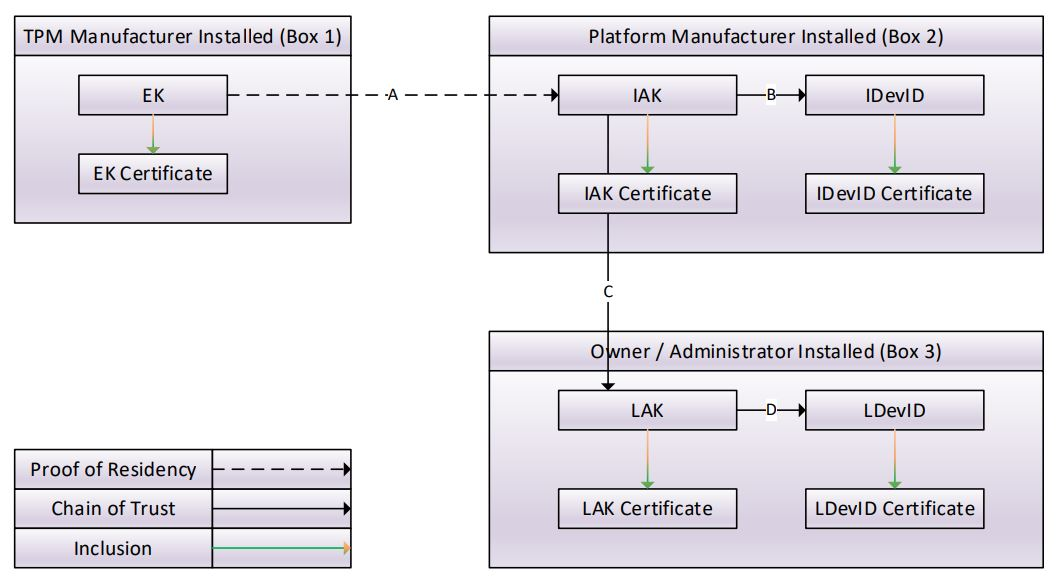
\includegraphics[width=\linewidth]{chap_3_figures/certificateRelationships.jpg}
  \par\end{centering}
  \caption{Key and Certificate Relationships \cite{DevIDSpec-TCG}}
  \label{fig:cert_rel}
\end{figure}
\vspace{2em}
\begin{itemize}[itemsep=0pt,parsep=0pt,partopsep=0pt]
  \item \textsf{Box 1}: The EK certificate is signed by the TPM Manufacturer's CA and binds the EK to a specific TPM.
  \item \textsf{Line A}: The IAK is verified by the OEM's CA to have the correct key properties and to be loaded on the same TPM as the EK.
  \item \textsf{Line B}: The IDevID is verified by the OEM's CA to have the correct key properties and to be loaded on the same TPM as the IAK.
  \item \textsf{Box 2}: The IAK certificate and IDevID certificate is signed by the OEM's CA and binds the IAK and IDevID to a specific device.
  \item \textsf{Line C}: The LAK is verified by the Owner's CA to have the correct key properties and to be loaded on the same TPM as the IAK.
  \item \textsf{Line D}: The LDevID is verified by the Owner's CA to have the correct key properties and to be loaded on the same TPM as the LAK.
  \item \textsf{Box 3}: The LAK certificate and LDevID certificate is signed by the Owner's CA.
\end{itemize}

\vspace{2em}
Since a key with the \verb|Restricted| attribute set has the ability to prove that some unknown key is loaded on the same TPM as itself, AK certificates are used as the requisite existing certificate in the provisioning of new DevIDs. Specifically this means that AK certificates may be parent nodes in a chain of certificates. Due to this result, a chain of certificates exhibits a tree structure.
%To demonstrate that some non-IAK DevID belongs to a specific device, one must provide the chain of certificates which links that DevID's certificate to the OEM-provided root certificate.
The underlying security implications provided by a chain of certificates is formed primarily by the protocols that create these certificates. Specifically, the Proof of Residency and Chain of Trust lines in Figure \ref{fig:cert_rel} are a direct consequence of the assurances provided by the respective certification protocols.

Although, Figure \ref{fig:cert_rel} shows the relationships between keys and certificates for exactly one of each DevID type, in practice, there often exists multiple of each DevID. Due to algorithm agility, an OEM usually installs multiple IAKs and IDevIDs with varying algorithms and sizes. IAKs are always directly linked to an EK, while IDevIDs are always directly linked to an IAK. On the other hand, LAKs and LDevIDs may be directly linked to any attestation key (i.e., an IAK or LAK). This means that an LAK certificate may be used in the provisioning of LDevIDs or additional LAKs producing an arbitrarily long chain of certificates. 
%All DevIDs (excluding IAKs) must be directly linked to an AK because the \verb|Restricted| attribute is necessary in proving that the new key resides in a specific TPM (i.e., the same TPM as the AK).

